\documentclass{article}
\usepackage[style=ieee]{biblatex}
\bibliography{references.bib}
\usepackage[utf8]{inputenc}
\usepackage{graphicx}
\usepackage{float}
\usepackage{listings}
\usepackage{algorithm}
\usepackage{algpseudocode}
\usepackage{amsmath}
	
\title{Evolutionary Algorithm for the Bonded Molecular Conformation Problem}
\author{Bennett Gale}
\date{August 2018}
\lstset{language=C++, basicstyle=\ttfamily}

\begin{document}
\maketitle
% \tableofcontents
% \pagebreak

\section{Introduction}

The model molecular energy minimisation problem involves the geometric
configuration of a chain of atoms in two dimensions, each connected by rigid
bonds of unit length, such that the total potential energy yielded by the sum of
individual Lennard-Jones potentials is globally minimised. The total potential
energy of the cluster is given by
$$V(r)=\sum^{N-1}_{i=1}\sum^{N}_{j=i+1}\left(r^{-12}_{ij}-2r^{-6}_{ij}\right)$$
Where $r$ is the euclidean distance between a pair of atoms and $N$ is the
number of atoms in the chain.

The energy minimisation problem is historically difficult because of the
exponential relationship between the locally stable structures and the number of
atoms, $N$, in the molecule. That is, as the size of the cluster increases, the
number of local minima increases exponentially such that when $N$ approaches
100, there exist more than $10^{140}$ minima \cite{DAVEN1996195}. It is
therefore necessary to employ sophisticated search algorithms in order to make
larger input sizes attainable.

Section~\ref{litreview} will discuss some of the research that has already taken
place in this area. Section~\ref{proposed} will detail the algorithm proposed by
this paper.

\section{Literature Review} \label{litreview}

Genetic algorithms have been applied \cite{doi:10.1002/qua.560440214,
PULLAN1998331, } successfully in order to extend the range of input size $N$
that is reachable through structural optimisation. This population based
approach emulates the Darwinian process of natural selection, and works by
performing crossover operations on pairs of candidate configurations with
selection probabilities based on their fitness, producing new child nodes which
contain genetic material from both parents. With every crossover operation there
is a small chance of subsequent random mutation of the child configurations, the
purpose of which is to promote genetic diversity within the population and
prevent premature convergence. Over many generations the population converges
towards a global minimum as each configuration communicates information about
the global search space through the crossover operation. This method has been
successful in producing results that were previously unseen in literature for
certain input sizes \cite{PULLAN1998331}.

Judson \textit{et al.} compare the performance of GAs with simulated annealing,
a probabilistic global optimisation technique in which Monte Carlo steps are
taken and new states are accepted if they are fitter, or with a probability
based on a function of a temperature value \cite{doi:10.1002/qua.560440214}.
When applied to the molecular conformation problem, they found that the GA
method and the SA method, both applied as global meta-heuristics in conjunction
with gradient-based local optimisers (conjugate gradient), similarly
outperformed purely stochastic methods \cite{doi:10.1002/qua.560440214}. Judson
\textit{et al.} classify points on the model energy surface as being in one of
three states: knotted and of high energy, unknotted and of low but not minimal
energy, and unknotted with globally minimised energy
\cite{doi:10.1002/qua.560440214}. They applied both GA and SA in order to make
the transition from the first state to the second state before applying local
optimisation to descend to the bottom of the basin.

Genetic operators for the two dimensional bonded Lennard-Jones problem have
since been further developed with successful results \cite{PULLAN1998331},
proving the GA approach to be a viable global optimisation technique. Pullan
\cite{PULLAN1998331} proposes three genetic crossover methods and four mutation
operators and applies these in a parallel genetic algorithm to find global
minima for most values of $N, 2 \leq N \leq 55$, as well as a minimum for $N =
61$ which was previously unseen in literature.

This two stage hybrid method has been successful, but Judson \textit{et al.}
also suggest the possibility of adding a third optimisation stage which is
intermediate between the global and local gradient methods
\cite{doi:10.1002/qua.560440214}. It is thought that a non-gradient optimisation
method such as the simplex method may provide a means of stepping over barriers
into possibly deeper minima surrounding those found by the global method in the
first phase.

More recently, the Conformational Space Annealing Method
\cite{PhysRevLett.91.080201} has been developed as a global optimisation
algorithm that has produced very good results when applied to the problem of an
unbound cluster of atoms with Lennard-Jones relationships. This algorithm
combines concepts of Monte Carlo with minimisation, genetic algorithms, and
simulated annealing. While this technique has not been applied to the bonded
variant of the Lennard-Jones conformation problem as discussed here, it
demonstrates that a hybrid approach combining SA and evolutionary population
based algorithms may be a viable technique in a similar problem domain.

\section{Proposed Algorithm} \label{proposed}

As discussed in section~\ref{litreview}, global meta-heuristics such as the
genetic algorithm, have been used successfully as a means of navigating the
global search space and avoiding local minima that are caused by knots in the
configurations \cite{PULLAN1998331, doi:10.1002/qua.560440214}. These methods
use the global optimiser to find unknotted potential candidate configurations
and then refine them using gradient-based methods. Judson \textit{et al.} have
suggested a three stage system in which a non-gradient optimiser such as the
simplex method may be used as an intermediate stage between the global and
local-gradient optimisation in order to traverse barriers into potentially
deeper basins \cite{doi:10.1002/qua.560440214}.

As simulated annealing has been found to be successful when combined with
evolutionary algorithms in similar problem domains \cite{PhysRevLett.91.080201},
this paper will explore its use as an intermediate non-gradient method such that
the proposed algorithm has three levels: global meta-heuristic (GA),
intermediate non-gradient optimisation (SA) and local gradient-based
optimisation (BFGS). The performance of this three stage optimisation method
will be compared with a purely evolutionary algorithm without the intermediate
step.

\subsection{Genetic Encoding}

Encoding each  molecule as a chain of two-dimensional Cartesian coordinates
would require constraints to be enforced so that the relative orientations and
unit length bonds are maintained. In order to avoid this, therefore, molecules
will be encoded as sequences of $N-2$ angles, where $N$ is the number of atoms
in the molecule and each angle, $\alpha_i$ represents the rotation of the
segment following atom $a_i$. This encoding scheme means that Cartesian
coordinates must be calculated at each Lennard-Jones potential computation as it
requires euclidean distances between pairs of atoms to be computed, but results
in much simpler crossover and mutation operations.

\subsection{Selection \& Crossover Methods}

% An elitist methodology will be utilised throughout the GA optimisation,
% meaning that the single fittest configuration will be passed on unmodified to
% subsequent generations in order to preserve beneficial traits and provide a
% mechanism for remembering information about the best configuration that has
% been found so far.

% Pairs of parents to be crossed over will then be selected using the Roulette
% method, where the probability for a potential parent to be selected is based
% on a function of its fitness value. The `elite' configurations that were
% inherited from the previous generation will also be candidates for selection
% using this method. Selected parents will undergo one of the following
% crossover operators with equal probabilities of occurring:

The population is represented as a large pool of size $n_{pop} \times 2$ where
$n_{pop}$ is the user-provided population size. This pool contains both the
current population and the generated children in a single array such that it
can be easily sorted based on fitness.

% \subsubsection{Single-Point Crossover}

% A single atom $a_i$ will be randomly selected. Atoms to the left of this point
% in one parent will form the left segment of the child, and the right segment
% of the child will be similarly formed from the atoms to the right of the
% second parent. A second child may be generated by repeating with the opposite
% segments (the right segment from parent one and the left segment from parent
% two). Finally, the angle $\alpha_i$ at the crossover point will be iterated
% through discrete steps until an angle is found which results in the lowest
% energy, as described by Pullan \cite{PULLAN1998331}.

\subsubsection{Crossover}

A single-point crossover operator is applied as follows: A single angle index
$a_i$ is selected at random. Angles to the left of this point in the first
parent form the left segment of the child, and the right segment of the child is
similarly formed from the atoms to the right of the second parent.

\paragraph{Partial L-BFGS}

Finally, $\alpha_i$ is locally optimised by applying BFGS with this single angle
as its only optimisation parameter, with the rest of the angles fixed. Energy
and gradients for use in the BFGS algorithm are computed using the entire
molecule, while only the subset is optimised, leaving the rest of the angles
unchanged. This optimisation of the single crossover point effectively locally
optimises the relative orientation of the two connected segments.

%TODO: Should I leave this paragraph in?
Crossover operators with multiple crossover-points were not found to be
beneficial during experimentation and were even detrimental in some cases. As
such, they have been excluded from this study. The focus is primarily on
evaluating the use of annealing as a mutation operator and therefore the
crossover operation has been kept simple.

\subsubsection{Selection}

Pairs of parent configurations to be crossed over are selected by choosing
randomly from the fittest half of the population. This is repeated $n_{pop}$
times so that the number of children created is equal to the population size and
forms the next generation. Selecting from the fitter half of the population
ensures that information about the global search space is retained through
multiple generations by providing bias towards states that are closer to the
global minimum.

At each generation the entire pool is sorted so that the $n_{pop}$ fittest
states, including children and fitter parents from the current generation move
to the top half of the pool. This forms the new generation's population, and
implicitly provides a form of elitism by allowing states from the previous
generation to remain in the population if they are fit enough. After sorting,
the second half of the pool contains discarded states which can be later
overwritten with new children during subsequent crossover stages.

\subsection{Mutation}

The mutation mechanism is where the intermediate non-gradient optimisation
algorithm will be incorporated. In traditional genetic algorithms, mutation has
a small chance of occurring and is random, resulting in some states which are
less fit in the hopes that this will later lead to a deeper basin in the search
space. By incorporating simulated annealing at the mutation stage it is hoped
that the configuration will be dragged in a downward direction while also
providing enough stochastic properties to allow boundaries between minima to be
traversed, which is the goal of any mutation operator.

\subsubsection{Mutation Rate} \label{mutationrate}

Mutation generally has a low chance of occurring so as not to corrupt fit
configurations too frequently and lose information provided by the global
search. It was found, however, that with a low mutation rate the search tended
to converge prematurely due to an overly homogeneous population. In order to
overcome this, the chance of mutation for each configuration is based on its
similarity to its direct neighbour. That is, each state is mutated if its
fitness is within one unit of that of the previous state.

Additionally, if a state's energy is positive it is guaranteed to be mutated.
This has the effect of reducing the number of knotted configurations in the
population, as the mutation operators tend to guide them towards a negative
energy state.

\subsubsection{Mutation Operators}

The following operators mutate a given configuration in both biased and
unbiased ways.

\paragraph{Unravelling}

This mutation operator is based on one described by Pullan \cite{PULLAN1998331}
in which A random angle index $\alpha_i$ is selected in the molecule and the
distance between this point and each endpoint is compared. The angles between
the selected angle and the closest end forms a new segment of angles. For each
angle in the selected segment, a very small (close to zero) random number is
chosen and the angle is set to that value. This results in one end of the
molecule being `unravelled' into a straight line, which effectively removes any
knots or kinks within that segment.The segment is later `rewound' through
subsequent local optimisation.

\paragraph{Guided Stochastic Mutation}


A random angle is selected and both the current fitness of the molecule and the
current value of this angle is stored.The selected angle is set to a random
value between $-\pi$ and $\pi$ and the fitness is recomputed. If the new fitness
is worse than the previous fitness, the angle is reverted to its previous state.
This process is then repeated until either the maximum number of iterations is
reached, or an improved configuration is found. This limit is important because
after many generations it becomes increasingly difficult to find a random change
in an angle that does not give lower energy, which would otherwise result in an
infinite loop.

\paragraph{Naive Mutation}

This is an unbiased mutation operator which simply selects a random angle
$\alpha_i$ and sets it to a random new value between $-\pi$ and $\pi$. This
operator has no regard for whether the mutation improves or worsens state, and
primarily serves the purpose of reducing homogeneity and premature convergence
within the population.

\paragraph{Annealed Mutation}

A relatively brief annealing schedule is used due to the fact that during every
iteration an energy computation is required. The goal at this intermediate
search algorithm is not to find the global minimum, but merely to provide a more
localised search for deeper basins in the vicinity of the current configuration;
it is hoped that if the GA search has found a local minimum in close proximity
to the global minimum, the SA stage will take large enough steps in order to
climb over the boundary into the neighbouring basin where it can be finally
optimised by the gradient search in the next stage. Therefore, an annealing
schedule that prioritises speed over optimality will be chosen. The initial
temperature $T$ will be set to 100 and decrement by one every iteration until it
reaches 0.

During annealing, random angles are selected and modified by random amounts. If
the change produces an improved state, it is always accepted. If the change
produces a worsened state, it is accepted with a probability of $1 - e^{-\Delta
E / Tk}$ such that both the current `temperature' as well as the degree to which
the change will worsen the configuration, determine whether the change is to be
accepted. $\Delta E$ represents the change in energy that will occur if the new
configuration is accepted, $T$ represents the current temperature, and $k$ is
used to scale probability curve. A value of $k=0.03$ was chosen as this provides
a reasonable probability curve for energy deltas of 1 and below.

\subsection{GA Procedure and Parameters}

The following GA parameters are used:
\begin{description}
	\item[Population Size] 12
	\item[Maximum Generations] 100
	\item[Mutation Rate] Deterministic and based on conditions as described in
	section~\ref{mutationrate}
\end{description}
The GA works by continually sorting a large pool (of size $n_{pop} \times 2$) of
configurations in order to rank them in order of fitness and subsequently select
states for crossover and mutation operators. The population is initialised with
random molecules and sorted and then the procedure outlined in REF are carried
out until either a known global optimum is found or the maximum number of
generations is reached.

%%%% GA Pseudocode here

The final stage of each GA iteration, after candidate configurations have been
found by the GA and its immediate vicinity has been further explored through
mutation, is to refine the configuration using gradient-based local search. This
stage uses the gradient of the objective function in order to guarantee that the
bottom of the current basin will be reached. The quasi-Newton method
Broyden–Fletcher–Goldfarb–Shanno (BFGS) will be applied at this stage resulting
in a fast descent towards the current local minimum at each stage. The
coordinates of this locally optimised configuration are also be passed back to
the GA so that improvements are retained in future iterations. This is known as
a `Lamarkian'process and has previously been found to be beneficial when used
with this problem \cite{doi:10.1002/qua.560440214}.

\section{Results}

\begin{figure}
	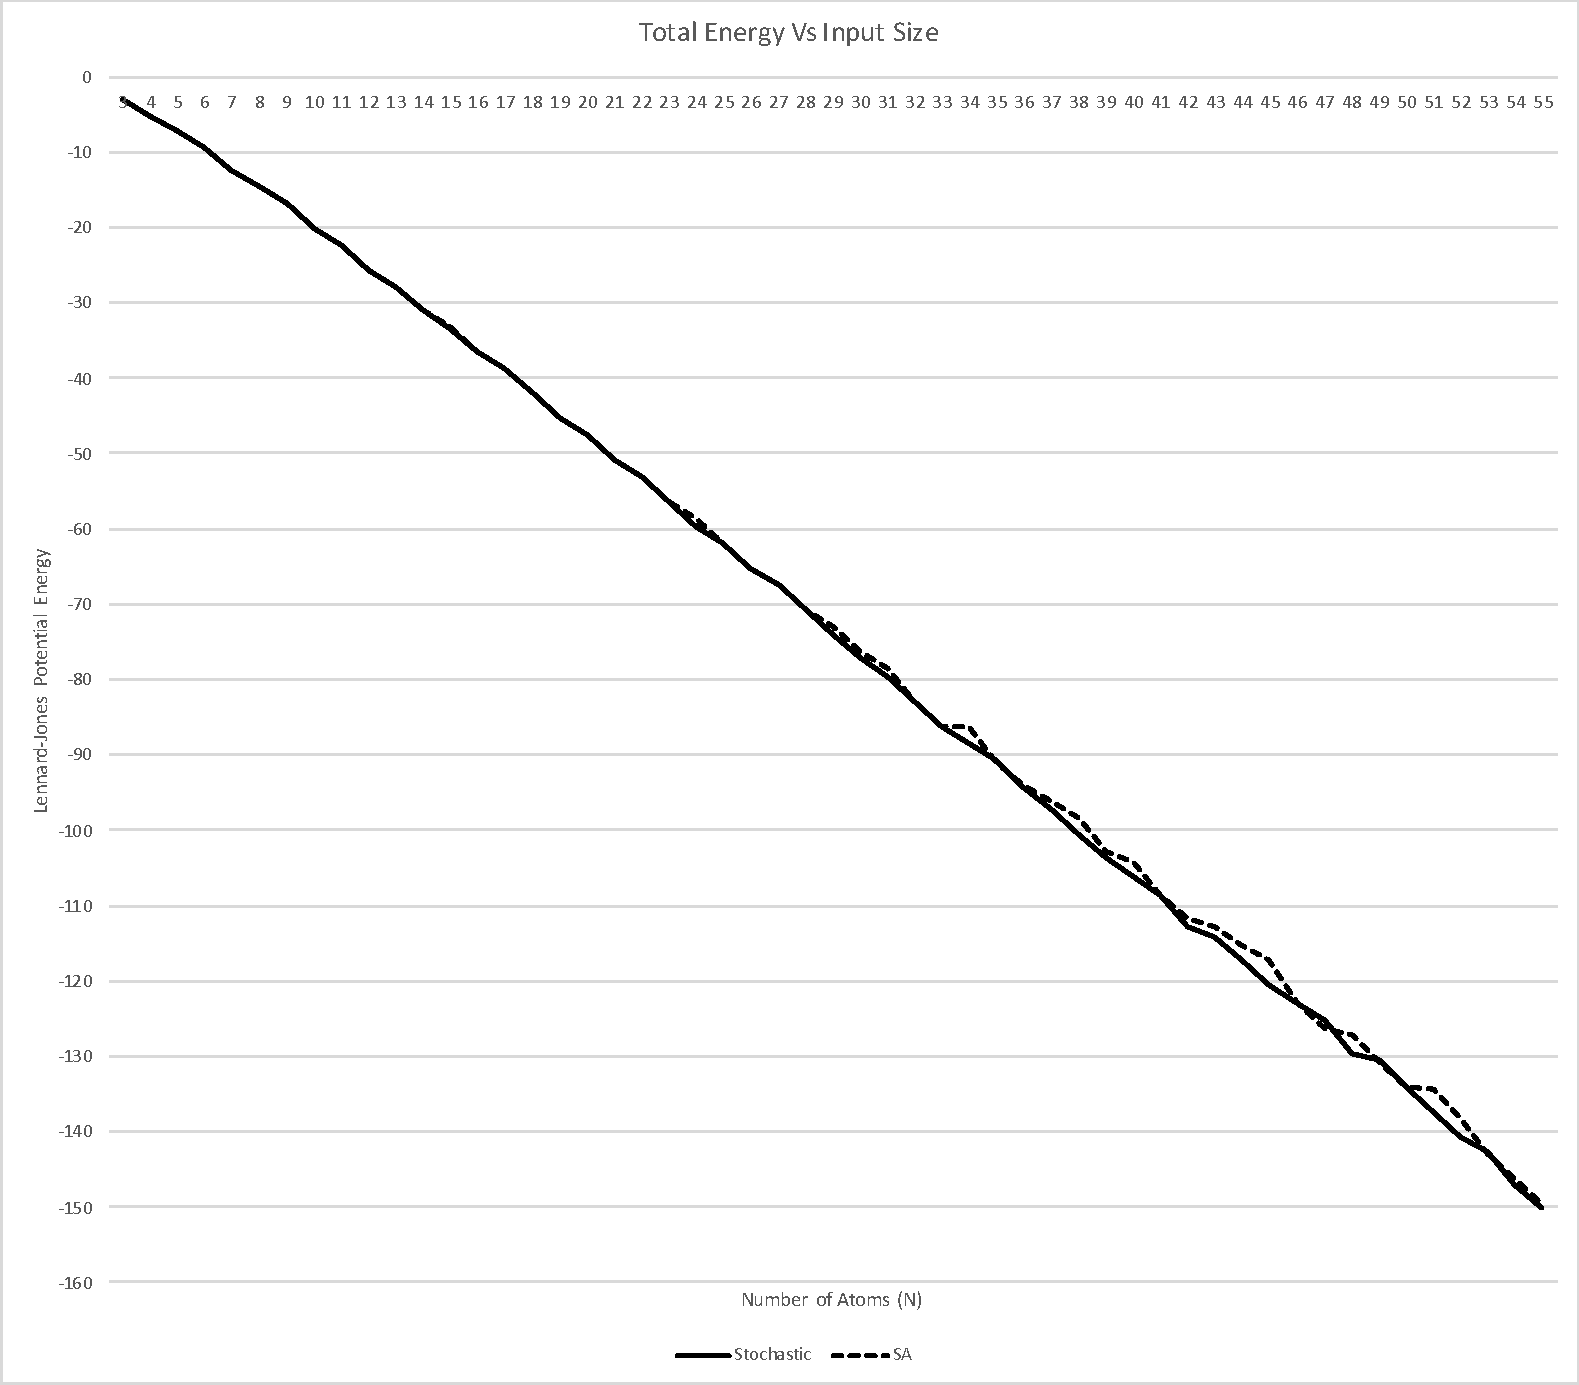
\includegraphics[width=\textwidth]{nvse.pdf}
	\caption{Lennard-Jones Potential as N size increases}
	\label{fig:nvse}
\end{figure}

\section{Conclusion}



\section{Appendix}

\begin{table}[]
	\label {tab:nosa}
	\centering
	\begin{tabular}{cccc|cccc}
	$N$  & Optimal & Found & Gen. & $N$  & Optimal & Found  & Gen. \\
	\hline
	3  & -3.0    & -3.0  & 0    & 30 & -77.3   & -77.2  & 89   \\
	4  & -5.1    & -5.1  & 1    & 31 & -79.5   & -79.6  & 70   \\
	5  & -7.2    & -7.2  & 1    & 32 & -82.9   & -82.9  & 88   \\
	6  & -9.3    & -9.4  & 52   & 33 & -86.1   & -86.2  & 87   \\
	7  & -12.5   & -12.5 & 67   & 34 & -88.4   & -88.5  & 99   \\
	8  & -14.7   & -14.7 & 75   & 35 & -91.7   & -90.7  & 99   \\
	9  & -16.9   & -16.9 & 0    & 36 & -95.0   & -94.1  & 89   \\
	10 & -20.1   & -20.1 & 0    & 37 & -98.3   & -97.3  & 98   \\
	11 & -22.3   & -22.3 & 99   & 38 & -100.6  & -100.6 & 88   \\
	12 & -25.6   & -25.6 & 96   & 39 & -103.8  & -103.7 & 86   \\
	13 & -27.8   & -27.8 & 21   & 40 & -107.2  & -106.0 & 79   \\
	14 & -31.0   & -31.0 & 95   & 41 & -109.4  & -108.5 & 96   \\
	15 & -33.2   & -33.3 & 78   & 42 & -112.8  & -112.7 & 98   \\
	16 & -36.5   & -36.5 & 5    & 43 & -116.0  & -114.1 & 97   \\
	17 & -38.7   & -38.7 & 79   & 44 & -119.4  & -117.3 & 93   \\
	18 & -42.0   & -42.0 & 77   & 45 & -121.6  & -120.6 & 96   \\
	19 & -45.3   & -45.3 & 87   & 46 & -125.0  & -122.9 & 87   \\
	20 & -47.5   & -47.6 & 76   & 47 & -128.6  & -125.3 & 94   \\
	21 & -50.8   & -50.8 & 89   & 48 & -131.6  & -129.5 & 95   \\
	22 & -53.0   & -53.1 & 99   & 49 & -133.8  & -130.4 & 78   \\
	23 & -56.3   & -56.4 & 74   & 50 & -137.2  & -134.0 & 93   \\
	24 & -59.6   & -59.6 & 90   & 51 & -140.5  & -137.4 & 72   \\
	25 & -61.9   & -61.9 & 91   & 52 & -143.7  & -140.7 & 95   \\
	26 & -65.1   & -65.1 & 22   & 53 & -146.1  & -142.6 & 98   \\
	27 & -68.4   & -67.4 & 97   & 54 & -149.3  & -147.0 & 99   \\
	28 & -70.7   & -70.7 & 53   & 55 & -152.7  & -150.0 & 68   \\
	29 & -74.0   & -74.0 & 77   &    &         &        &      \\

	\hline 
	\end{tabular}
	\caption{Results with unravelling, guided stochastic, and stochastic
	mutation
	operators}
 \end{table}

 \begin{table}[]
	\label {tab:yessa}
	\centering
	\begin{tabular}{cccc|cccc}
	$N$  & Optimal & Found & Gen. & $N$  & Optimal & Found  & Gen. \\
	\hline
	3  & -3.0    & -3     &    0   & 30 & -77.3   & -76.3    &  89  \\
	4  & -5.1    & -5.1   &    0   & 31 & -79.5   & -78.5    &  81  \\
	5  & -7.2    & -7.2   &    23  & 32 & -82.9   & -82.9    &  95  \\
	6  & -9.3    & -9.4   &    90  & 33 & -86.1   & -86.2    &  98  \\
	7  & -12.5   & -12.5  &    90  & 34 & -88.4   & -86.2    &  93  \\
	8  & -14.7   & -14.7  &    93  & 35 & -91.7   & -90.8    &  99  \\
	9  & -16.9   & -16.9  &    2   & 36 & -95.0   & -94.0    &  95  \\
	10 & -20.1   & -20.1  &    1   & 37 & -98.3   & -96.2    &  86  \\
	11 & -22.3   & -22.3  &    53  & 38 & -100.6  & -98.5    &  90  \\
	12 & -25.6   & -25.6  &    80  & 39 & -103.8  & -102.7   &  94  \\
	13 & -27.8   & -27.8  &    24  & 40 & -107.2  & -104.2   &  61  \\
	14 & -31.0   & -31.0  &    56  & 41 & -109.4  & -108.5   &  87  \\
	15 & -33.2   & -33.23 &    73  & 42 & -112.8  & -111.7   &  95  \\
	16 & -36.5   & -36.5  &    15  & 43 & -116.0  & -112.8   &  90  \\
	17 & -38.7   & -38.8  &    72  & 44 & -119.4  & -115.2   &  92  \\
	18 & -42.0   & -42.1  &    93  & 45 & -121.6  & -117.3   &  99  \\
	19 & -45.3   & -45.3  &    94  & 46 & -125.0  & -123.0   &  96  \\
	20 & -47.5   & -47.5  &    86  & 47 & -128.6  & -126.3   &  88  \\
	21 & -50.8   & -50.8  &    22  & 48 & -131.6  & -127.2   &  77  \\
	22 & -53.0   & -53.0  &    61  & 49 & -133.8  & -130.7   &  67  \\
	23 & -56.3   & -56.4  &    92  & 50 & -137.2  & -134.0   &  83  \\
	24 & -59.6   & -58.7  &    76  & 51 & -140.5  & -134.2   &  98  \\
	25 & -61.9   & -61.9  &    70  & 52 & -143.7  & -138.3   &  98  \\
	26 & -65.1   & -65.1  &    3   & 53 & -146.1  & -142.9   &  45  \\
	27 & -68.4   & -67.4  &    79  & 54 & -149.3  & -146.3   &  85  \\
	28 & -70.7   & -70.7  &    67  & 55 & -152.7  & -149.5   &  97  \\
	29 & -74.0   & -73.0  &    90  &    &         &          &       \\

	\hline 
	\end{tabular}
	\caption{Results with unravelling, guided stochastic, and annealed mutation
	operators}
 \end{table}

 \begin{figure}
	\includegraphics[width=\textwidth]{figs/combined1.png}
	\caption{Best Solution Found for N=5 to N=30}
	\label{fig:combined1}
\end{figure}

 \begin{figure}
	\includegraphics[width=\textwidth]{figs/combined2.png}
	\caption{Best Solution Found for N=35 to N=55}
	\label{fig:combined2}
\end{figure}


%\subsection{Implementation}

% \begin{algorithm} \caption{Proposed High-Level Algorithm} \label{algorithm}
%   \centering \begin{algorithmic} \Procedure{optimise}{} % \State $nn \gets new
%   Network$ %   \For{$i \gets 0; i <= number\_of\_epochs; i++$} %
%   \For{$\textit{each data partition of minibatch size}$} %           \State
%   $\textit{Do forward pass}$ %           \State $\textit{Backpropagate the
%   resulting error}$ %           \State $\textit{Update the weights
%   proportionally to their contribution to the error}$ %       \EndFor %
%   \State $\textit{Shuffle and repartition the data}$ %   \EndFor \State $P
%   \gets \textit{Initial Population Size}$ \State $population \gets initialise$
%   \EndProcedure \end{algorithmic}
	
% \end{algorithm}

\pagebreak

\printbibliography

\end{document}